\chapter{Conception et construction des bâtiments}

Ce premier chapitre ouvre la thèse en présentant les différentes phases de la construction d'un projet de bâtiment. Ces phases sont aujourd'hui normées et chaque acteur de la construction a un rôle bien déterminé dans ce processus. La liste suivante présente alors ces étapes et les acronymes utilisés:

\begin{enumerate}
  \item Étudier la faisabilité du projet architectural et autorisation. Le maître d'ouvrage rencontre un architecte et un programmiste pour réaliser les études d'avant projet: ESQ (Etudes d'esquisses), APS (Avant-Projet Sommaire), APD (Avant-Projet Définitif) et DPC (Dossier de demande de Permis de Conduire)
  \item Conception détaillée du bâtiment: PRO (Études de PROjet)
  \item Planification de la construction: DCE (Dossier de Consultation des Entreprises) et plans d'exécution
  \item Sélection des entreprises de la construction: ACT (Assistance aux Contrats de Travaux)
  \item Chantier: DET (Direction de l'exécution des travaux) et OPC (Ordonnancement, coordination et Pilotage du Chantier)
  \item Livraison du bâtiment au maître d'ouvrage: AOR (Assistance aux Opérations de Réception)
\end{enumerate}

Cette liste montre d'une part la chronologie des différentes phases de la conception des bâtiments et nous permet d'autre part d'avancer qu'une gestion intégrée de ces étapes peut améliorer l'efficacité de la construction. Cela passe par une implication davantage holistique des bureaux d'études, artisans, entreprises de construction, exploitant et occupant dès les premières phases du projet.

Du point de vue du bureau d'études thermique et environnement, la conception ou la rénovation de bâtiments, rime avec évaluation des performances futures des constructions. Concernant l'environnement, nous verrons dans ce chapitre que des certifications permettent d'aller au-delà des exigences du code de l'environnement. A propos de l'énergétique, nous verrons que se sont les labels énergétiques qui permettent dépasser les exigences de performances en comparaison à la règlementation thermique. L'évaluation de ses niveaux de performance a été accompagné d'outils permettant de les quantifier. Nous nous intéressons ici particulièrement à la Simulation Thermique Dynamique (STD) qui est de plus en plus intégrée au processus de conception des bâtiments et qui permet théoriquement de modéliser son fonctionnement réel. Une comparaison de ces outils est proposé dans ce chapitre.

\section{Modélisation numérique des bâtiments}

Pourquoi modélise t-on les bâtiments?
- Outil d'aide à la conception. Comme les trois piliers du développement durable, l'objectif est de trouver un optimum économique, social et environnemental. Détailler les 3 piliers.

\section{Calculs conventionnels}

Afin de créer un seuil minimum de performance énergétique des bâtiments, la législation a mis en place des réglementations thermiques évolutive. La première réglementation fait suite au premier choc pétrolier de 1973 qui a déclenché une prise de conscience de la nécessité d'économiser l'énergie. Sa mise en place concerne les bâtiments neufs et date de 1974. Aujourd'hui, la Règlementation Thermique (RT) en vigueur est la RT 2012, elle précède la future RT 2020 et s'inscrit dans la continuité des RT 2005, 2000, 1988 et 1974 aux exigences croissantes. Depuis 2000, ces règlementations thermiques expriment des exigences sur les résultats en énergie primaire, alors que les RT antérieures imposent des exigences de moyens, d'où leur absence sur la Figure \ref{fig:Evolution_des_performances_des_rt}. En effet, bien que depuis 1974 les performances s'améliorent, une comparaison quantitative des deux premières RT n'est pas significative avec les dernières. Impulsé par le Grenelle de l'Environnement les acteurs du bâtiment se préparent à une nouvelle évolution significative des performances pour la RT 2020. Outre des améliorations techniques des matériaux, la RT 2020, ou plutôt la Règlementation Bâtiment Responsable (RBR) devrait également prendre en considération les usages de l'électricité spécifique (appareils ménagers, boxes, TV, etc.), l'énergie grise des constructions ainsi que de la mobilité qui est liée à la densité urbaine environnante. En effet, ces paramètres ne sont actuellement pas pris en considération dans la RT 2012 qui ne s'intéresse qu'à 5 postes de consommations (chauffage, climatisation, eau chaude sanitaire, éclairage et auxiliaires).

\begin{figure}[h]
\centering
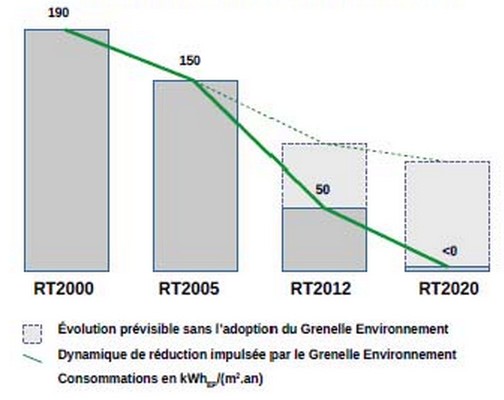
\includegraphics[scale=0.7]{Images/Evolution_des_performances_des_rt}
\caption{Évolution des exigences réglementaires de consommation énergétique des bâtiments neufs: une rupture opérée par le Grenelle Environnement. Source: Ministère de l'écologie, du développement durable et de l'énergie}
\label{fig:Evolution_des_performances_des_rt}
\end{figure}

La méthode de calcul actuelle Th-BCE 2012 n'a pas pour vocation de faire des calculs de consommations réelles, elle utilise comme données d'entrée tous les éléments descriptifs du bâtiment et de ses équipements. Les éléments apportés après la réception du bâtiment ainsi que les paramètres indépendants du bâtiment intervenant dans la méthode sont définis de façon conventionnelle: il s'agit notamment des données climatiques et celles relatives à l'usage des bâtiments. Il est alors possible de confirmer que les bâtiments sont aux normes thermiques et qu'ils peuvent effectivement être construits ou encore de comparer les bâtiments les uns aux autres d'un point de vue thermique et énergétique sans que l'ingénieur d'étude n'ait à priori d'impact sur les résultats et donc la conformité.

Plusieurs logiciels ont été développés en suivant le moteur de calcul Th-BCE 2012, lui même développé par le CSTB afin de vérifier la conformité d'un projet à la RT2012. Sans détailler les caractéristiques de ces logiciels, les plus répandus en France sont Pleiades+COMFIE, Perrenoud, Clima-Win, DesignBuilder et CYPE.

Le prochain chapitre évoque les labels et certifications et montre alors qu'il est fréquent que les maîtres d'ouvrage éprouvent la volonté de construire des bâtiments plus performants que ce que les règlementations fixent. Le chapitre d'après traite lui des Simulations Thermiques Dynamiques qui ont plus de flexibilité que les calculs règlementaires et qui permettent aussi des évaluations dans le cadre de labelisations et certifications.

\section{Labels et certifications}

Locomotive des projets innovants et performants. Ils recherchent la qualité environnemental...

Les certifications et labels sont des signes de qualité des bâtiments permettant de les catégoriser selon les modes de construction et les performances. Les certifications garantissent une construction ou une rénovation des bâtiments (maisons, immeubles, crèches, bureaux, ...) respectant de strictes exigences en termes de confort, santé, maîtrise des charges et environnement. Les labels valorisent uniquement la performance énergétique des bâtiments, sans tenir compte des autres éléments (biodiversité, qualité de l'air, durabilité). La diversité des certifications et labels donnent la possibilité aux constructeurs puis aux futurs acquéreurs de choisir un logement répondant à leurs priorités et souhaits. Ainsi une certification couvre plus de champ qu'un label qui ne s'intéresse qu'à la dimension énergétique et qui ne peut être demandé qu'au sein d'une certification.

Plusieurs démarches ont été initiées dans les pays européens pour améliorer et codifier les démarches constructives. Les principes de l'éco-construction peuvent se décliner en France avec la certification de construction Haute Qualité Environnementale (HQE), définissant 14 cibles dans 4 domaines (éco-construction, eco-gestion, confort et santé) ou la certification \textit{BRE Environmental Assessment Method} BREAM, organisée autour de 10 catégories (gestion, bien-être et santé, énergie, transport, matériaux, eau, déchets, paysage et écologie, pollution et innovation). Les labels, tels qu'Effinergie ne peuvent être obtenus qu'après certification et intègrent donc également les principes de l'éco-construction. Les labels et certifications ne sont pas une spécificité française, en effet on peut retrouver Minergie en Suisse, Passivhaus en Allemagne, LEED en Amérique du Nord. En 2016, le label Bâtiment Bas CArbone (BBCA) a vu le jour afin d'évaluer l'empreinte carbone des opérations. Pour obtenir ce label un effort particulier doit être fait sur la construction elle-même. En effet, avec l'amélioration des performance énergétique des bâtiments en phase d'exploitation, une part très importante des émissions de gaz à effet de serre à lieu en phase de chantier. Ce label BBCA récompense alors les opérations qui utilisent des matériaux bio-sourcés et locaux ainsi que les chantiers qui recyclent leurs déchets.

Les intérêts de vouloir construire des bâtiments au delà des règlementations sont multiples. D'une part, cela apporte une visibilité au bâtiment car il mobilise des technologies nouvelles qui attisent la curiosité d'autres maîtres d'ouvrage et rendent donc le bâtiment désirable. Dans le domaine public les certifications peuvent être accompagnées de subventions ce qui permet de limiter d'éventuels sur-coûts. Aussi, par définition un bâtiment certifié ou labellisé est plus performant que la moyenne et réduira donc ses coûts d'exploitation pour un confort d'habitat à priori également amélioré. Un bâtiment certifié renvoie aussi à l'assurance que les meilleures pratiques de construction ont été intégrées au chantier. Alors que cette assurance de qualité, qui est une marque de reconnaissance, est sensée être recherchée par les maîtres d'ouvrage pour une future valorisation lors de la vente ou lors de la cession du bâtiment, il apparaît que l'aspect économique inhibe bien souvent les bonnes volontés environnementales. La certification aborde les problèmes environnementaux dans leur globalité et permet aux promoteurs et concepteurs immobiliers d'amener de l'objectivité à la performance environnementale vis à vis de leurs clients.

La présentation des labels et certifications dans ce manuscrit se justifie par le fait que pour les attribuer il est nécessaire d'utiliser des logiciels qui quantifient les variables d'intérêts. La certification HQE impose par exemple des calculs d'éclairage, d'ensoleillement, d'Analyse de Cycle de Vie (ACV) et de calculs thermiques. Les calculs thermiques sont réalisés avec des logiciels de Simulations Thermiques Dynamiques (STD) afin de tester les comportements du bâtiment. La présentations de ce type de logiciel est le sujet de la section suivante, mais il est dès maintenant notable qu'ils ne sont pas exclusivement utilisés dans le cadre de certifications et labels, loin de là.

\section{Logiciels de Simulations Thermiques Dynamiques}

Évaluer les besoins annuels de chauffage ou de rafraîchissement d'un bâtiment requiert de disposer de très nombreuses données permettant de décrire précisément l'enveloppe du bâtiment, les conditions météorologiques et l'usage du bâtiment. À partir de ces éléments, il est possible d'appliquer les lois de la thermique propres aux différents types d'échanges thermiques (convection, conduction, rayonnement) pour en déduire les puissances instantanées mises en jeu. Pour obtenir des résultats théoriques proches des résultats réels, les logiciels de Simulation Thermique Dynamique (STD) permettent de considérer l'ensemble des paramètres influant à chaque pas de temps de la simulation. Les prochains paragraphes présentent des logiciels du domaine privé et de la recherche. Pleiades+COMFIE, DYMOLA, EnergyPlus , ESP-r , IDA-ICE et TRNSYS sont les logiciels qui ont à un moment donné retenu notre attention pour la réalisation de cette thèse et sont alors présentés en détails dans ce qui suit. Le potentiel d'amélioration est également évoqué pour chaque logiciel à travers des travaux de recherche significatifs. Beaucoup d'autres logiciels existent pour modéliser et simuler les bâtiments dans leur environnement mais ne sont pas présentés ici: Virtual Environment, DOE, Climawin ou encore ArchiWizard parmi les plus répandus.

Avec l'accroissement des exigences de performances énergétiques et environnementales sur les nouveaux bâtiments, la STD est de plus en plus intégrée au processus de conception des bâtiments. Cela ne l'empêche pas d'être également appropriée dans des projets de rénovation, qui sont souvent plus difficiles à gérer car les informations concernant le bâti existant ne sont pas toujours disponibles. Par ailleurs, les Simulations Thermiques Dynamiques sont utilisées aussi bien pour le confort d'été que d'hiver car elles permettent d'évaluer les températures horaires dans différentes zones thermique des bâtiments. Les STD permettent d'estimer les besoins réels théoriques d'énergie à condition de bien connaître l'usage et cela le plus souvent au pas de temps horaire. De nombreux logiciels ont été développés afin de simuler un système, ici un bâtiment, qui n'est pas à l'équilibre.

\subsection*{simplifiés}

Dans le cadre de projets nécessitant une simulation thermique dynamique pour une application particulière, il peut être nécessaire de développer son propre outil. Kampf et Robinson \cite{Kampf-07} ont développé un modèle simple basé sur des équivalences électriques, cinq résistances et deux capacités afin d'étudier les flux de chaleur dans le bâtiment. Le principe de cette approche est basé sur une analogie entre la thermique et l'électricité. Le bâtiment est assimilé à un circuit électrique où les résistances électriques représentent les résistances thermiques (murs, fenêtres, toit, sol) et les capacités représentent l'inertie du bâtiment. Ce modèle électrique, 5R2C, a été repris par Darakdjian \cite{Darakdjian-13} de l'Ecole des Mines de Nantes pour réaliser une étude de STD des bâtiments à l'échelle du quartier urbain. Pour cela, le modèle simplifié de Kampf et Robinson est couplé à un outil de Système d'Information Géographique (SIG) développé par l'Institut de Recherche en Science et Techniques de la Ville (IRSTV): OrbisGIS. Cela permet d'obtenir en sortie des informations géo-localisées sur les performances des bâtiments à l'échelle du quartier. Les résultats absolus sont certes moins fiables que des logiciels spécialisés mais adaptables et viables en temps de calcul.

Dans le cadre de la garantie de performance énergétique, ces logiciels simplifiés ne permettent pas d'obtenir des résultats pouvant être contractualisés, car ils sont incomplets pour une étude globale et non validés par les autorités compétentes, tel que le CSTB. On comprend alors aisément que l'utilisation de logiciels commercialisés, comme ceux des prochaines sous-sections sont plus appropriés à une démarche de fiabilité de résultats. Cette section peut paraître surprenante ici, mais montre surtout que pour répondre à un objectif donné, il faut savoir trouver ou créer un outil adapté.

\subsection*{Pleiades+COMFIE}

L'outil de simulation thermique dynamique, COMFIE, est développé par l'école des Mines de Paris et l'interface Pleiades par IZUBA Énergies. L'ensemble Pleiades+COMFIE se démarque de beaucoup de logiciel de STD par l'ergonomie de l'interface utilisateur et à stabilité du logiciel. Aussi, la qualité de l'assistance technique participe à ce que le logiciel soit en France le plus utilisé par les bureaux d'études thermique. Le logiciel Alcyone, également développé par IZUBA, a été incorporé à Pleiades+COMFIE afin de réaliser la saisie graphique et de visualiser un rendu en trois dimensions. En sortie de simulation, l'exploitation de résultats est à un niveau avancé avec notamment des diagrammes de Sankey ou des zones de Brager générables.
Bien que Pleiades+COMFIE soit fortement apprécié par les utilisateurs en bureau d'études pour son confort d'utilisation, l'accessibilité au cœur du logiciel est nulle. Ainsi, dans un cadre de recherche, l'utilisation de Pleiades+COMFIE permet des études de sensibilité, mais empêche toute extension ou développement de modules, qui est réservé aux développeurs d'IZUBA. 

A ce propos, Vorger et al. \cite{Vorger-14} des Mines ParisTech ont travaillé sur l'amélioration de la prise en compte du comportement humain dans le logiciel en intégrant les activités des occupants par une modélisation stochastique. Ce travail consiste à générer aléatoirement des ménages et leurs équipements en ce basant sur des données statistiques de l'Institut National de la Statistique et des Etudes Economiques (INSEE). A partir de la génération de ces ménages les activités de chaque occupant sont également générés, ce qui permet d'y associer des consommations énergétiques. En réalisant plusieurs simulations, l'aspect stochastique de l'étude permet alors d'obtenir une fourchette de consommations, qui aide à s'engager dans le cadre d'un processus de Garantie de Performance Energétique (GPE) avec un risque d'erreur réduit.

\subsection*{DYMOLA}

\textit{DYnamic MOdelling LAboratoy} (DYMOLA) est un outil de modélisation et simulation, orienté R\&D et développé par Dassault Systèmes. Il permet de modéliser de manière pratique des systèmes dynamiques complexes sans se limiter au domaine du bâtiment. Bien que d'un intérêt limité dans notre cas, DYMOLA peut également permettre de modéliser des systèmes hydrologiques, électriques, ou encore relatifs au transport routier. Encore relativement peu utilisé dans le secteur du bâtiment, il est tout de même apprécié pour la description des systèmes énergétiques. En plus de la bibliothèque standard qui couvre plusieurs domaines d'ingénierie, les utilisateurs peuvent créer leurs propres bibliothèques de modèles pour leurs besoins spécifiques. 

Michaelsen et Eiden \cite{Michaelsen-09} ont développé la leur pour la prédiction du confort de l'occupant en se basant sur les travaux danois de Fanger, reportés par Charles \cite{Charles-03} sur les votes moyens prévisibles (\textit{Predicted Mean Vote} en anglais).

Gaaloul \cite{Gaaloul-12} pour sa thèse a étudié l'interopérabilité de la simulation dynamique du bâtiment en couplant plusieurs outils. Pleiades+COMFIE est dédié à la modélisation de l'enveloppe, TRNSYS à la simulation des systèmes énergétiques du bâtiment, MATLAB/Simulink pour le contrôle de la simulation, BRAHMS pour la simulation du comportement des occupants (cf Section \ref{BRAHMS}) et enfin DYMOLA pour la modélisation avancée de la VMC double flux. Ainsi, les trois outils de STD, dont DYMOLA, sont couplés entre eux mais également à un modèle du comportement des occupants, BRAHMS.

\subsection*{EnergyPlus}

EnergyPlus, développé en Fortran par le département de l'énergie des Etats-Unis d'Amérique, est un des logiciels de simulation énergétique le plus connu dans le monde \cite{Sousa-13} et le plus utilisé par les chercheurs de l'Annexe 66, \textit{Definition and Simulation of Occupant Behavior}. EnergyPlus découle de la fusion de DOE et BLAST, deux logiciels qui ne sont plus développés. EnergyPlus est un logiciel de simulation autonome dépourvu d'interface graphique. Des interfaces comme celle de DesignBuilder ont été intégrée pour exploiter le potentiel du cœur de calcul dans un environnement convivial. Le couple DesignBuilder/EnergyPlus permet de réaliser des calculs règlementaires, des certification LEED, des simulations énergétiques, des calculs aérauliques, des calculs d'éclairement et même de coûts global. Aussi, il existe un module d'optimisation permettant de déterminer les paramètres du bâtiment offrant le meilleur compromis coût, confort et impact environnemental. Ainsi, EnergyPlus est considéré comme l'outil le plus complet du marché, tout en étant gratuit et totalement flexible.

Jacob Chapman et al. \cite{Chapman-14} de l'Université de Nottingham ont développé une plateforme multi-agents à base de modèles stochastiques qui se couple avec le logiciel de STD, EnergyPlus. Cette plateforme n'est pas détaillée dans cette section puisqu'elle a été reprise comme base de travail pour cette thèse. La présentation de cette plateforme, nommée \textit{Multi-Agent Stochastic Simulation} (MASS) se trouve en Chapitre \ref{MASS}.

\subsection*{ESP-r}

ESP-r est un logiciel de STD \textit{open-source} créé et développé par l'Université de Strathclyde, en Ecosse, qui fonctionne sous Linux, qui est gratuit et dont le code source est libre. En plus de modéliser les performances thermiques, il peut modéliser les performances visuels et acoustiques ainsi que les émissions de gaz associés. Les évolutions récentes du logiciel permettent également de modéliser l'aéraulique et l'humidité. ESP-r peut informer l'utilisateur sur les possibilités d'optimisation des performances du bâtiment. L'aspect totalement ouvert du logiciel permet d'une part aux utilisateurs d'accéder au cœur des algorithmes et d'en modifier les propriétés et d'autre part d'échanger avec des programmes extérieurs. Un inconvénient relevé d'ESP-r est le manque de détails et de documentations pour les utilisateurs lors de modélisations complexes.

Pour sa thèse de doctorat Bourgeois \cite{Bourgeois-05} l'a utilisé afin de simuler l'ensemble des interactions bâtiment-systèmes-environnement, afin d'en quantifier l'influence sur les besoins énergétiques. Bourgeois utilise le module SHOCC (\textit{Sub-Hourly Occupancy Control}) qui permet d'étudier les phénomènes relatifs aux comportements des occupants dans les bâtiments. SHOCC couplé à ESP-r gère alors la position des stores et les besoins des occupants concernant le chauffage. Ce modèle a par la suite été repris par Hoes et al. \cite{Hoes-09} dans le but d'améliorer la finesse de modélisation de la présence des occupants dans l'espace. Ce modèle baptisé USSU (\textit{User Simulation of Space Utilization}) a alors été associé à la paire SHOCC/ESP-r pour démontrer que les activités des occupants doivent être évaluées en détails pour que les estimations des performances des bâtiments gagnent en fiabilité.

\subsection*{IDA-ICE}

Contrairement à Comfie+Pleiade qui apparait comme une boîte noire pour l'utilisateur, mais comme DYMOLA, EnergyPlus et ESP-r, le logiciel IDA-ICE est totalement ouvert aux modifications avec la possibilité d'accéder au cœur des composants du logiciel. Il permet l'utilisation des modèles BIM (Maquette numérique du bâtiment) notamment générés, par ArchiCAD ou Revit.

Le projet européen Tribute \cite{TRIBUTE-15}, utilise IDA-ICE, et a également pour objectif de diminuer le \textit{performance gap} (cf Section \ref{performance gap}) en affinant la modélisation du comportement des occupants, en revisitant les modèles des systèmes et en considérant le vieillissement des matériaux et équipements. Pour ce projet, des bâtiments sont monitorés ce qui permet de détecter en temps réel les défauts de performance énergétique des bâtiments en vue d'actions correctives, modélisées sous IDA-ICE.

\subsection*{TRNSYS}

TRaN SYstem Simulation (TRNSYS) program est un environnement complet de simulation des systèmes énergétiques développé par l'Université de Wisconsin-Madison au Etats-Unis depuis 1979. Ce logiciel permet d'intégrer toutes les caractéristiques du bâti mais aussi des systèmes de chauffage ou de climatisation afin de réaliser des simulations thermiques dynamiques. L'outil est basé sur une approche systémique des problèmes que l'on cherche à modéliser. Les modèles sont couplés entre eux par les interconnexions entre des entrées et des sorties de modules (appelés types). A l'image d'EnergyPlus, ESP-r, DYMOLA ou IDA-ICE l'accessibilité au cœur de calcul est bonne et le développement de modules annexes libres. La limite principale de TRNSYS est de ne pas pouvoir se connecter avec AutoCAD, ArchiCAD ou Revit pour l'importation et l'exportation de fichiers contrairement aux trois autres logiciels. Le bâtiment doit alors être dessiné sous Google Sketchup puis importé.

Bonte \cite{Bonte-14} a développé un modèle basé sur le confort thermique et visuel des occupants, à l'Université de Toulouse, qu'il a intégré au logiciel TRNSYS-17. Ce modèle nommé OASys (\textit{Occupants’ Actions System}) permet alors de prendre en compte les préférences interindividuelles et permet la simulation des actions des occupants, en fonction de leurs sensations thermiques ou visuelles sur différents moyens d'actions tels que: la température de consigne, les stores, les fenêtres, l'éclairage ou la tenue vestimentaire. Ce modèle du comportement de l'occupant par intelligence artificielle fonctionne en deux phases: une phase d'apprentissage et une phase d'exploitation ou les agents réalisent les actions qui leur permettent d'améliorer leur confort.

\subsection*{Comparaison}

Le Tableau \ref{Tab:Synthese_logiciels_STD} synthétise les points forts et faiblesses de chacun de ces outils de simulations thermiques dynamiques en mixant les points de vu de l'ingénierie avec ceux de la recherche.

\begin{table}[h]
\centering
\begin{tabular}{|p{3.5cm}||p{5.75cm}|p{5.75cm}|}
\hline Logiciels & Points forts & Points faibles \\
\hline
\hline Logiciels simplifiés & Personnalisé \newline Rapide en temps de calcul & Non certifiés donc non fiables \newline Investissement de développement lourd \\
\hline Comfie+Pleiade & Convivialité de l'interface \newline Large utilisation des BET français & Flexibilité \newline Coût \\
\hline DYMOLA & Simulation Multi-Ingénierie \newline Flexible & Peu utilisé en BET \newline Coût \\
\hline EnergyPlus & Gratuit \newline Flexible & Pas d'interface libre \newline Peu utilisé en France \\
\hline ESP-r & Gratuit \newline Flexible \newline Optimisation de projet automatisé & Manque de documentation \newline Peu utilisé en France \\
\hline IDA-ICE & Flexibilité \newline Interface conviviale & Peu utilisé en France \newline Coût \\
\hline TRNSYS & Flexibilité \newline Modélisation systèmes  & Interface peu conviviale \newline Gestion des géométries \newline Coût \\
\hline 
\end{tabular}
\caption{Tableau comparatif des logiciels de STD}
\label{Tab:Synthese_logiciels_STD}
\end{table}

\section{Optimisation du management de projet}

Comme nous l'avons vu, concevoir des bâtiments implique de posséder des outils qui soient à la hauteur des ambitions fixées. Le choix du logiciel de simulation énergétique pour la recherche est fondamental car tous n'offrent pas les mêmes libertés et possibilités, mais ce choix l'est également dans le cadre des projets d'ingénierie. En effet, selon les spécificités des bâtiments étudiés, certains logiciels peuvent se révéler plus pertinent que d'autres. A titre d'exemple et  sans rentrer dans les détails, certains logiciels gèrent mieux que d'autres le zonage, les usages ou l'hygroscopie des matériaux.

Ainsi, choisir des outils appropriés en fonction des projets est essentiel dans l'acte de construire, néanmoins cela n'est réellement efficace que si la gestion de projet en elle même est coordonnée entre les différents acteurs. Cette section présente trois notions montantes afin d'optimiser le management de projet de construction: la maquette numérique, la démarche de conception intégrée et le commissionnement (présenté en détails en Section \ref{Engagement performantiel - Technique}).

La maquette numérique, ou plus communément appelé BIM, pour \textit{Building Information Modeling} est un modèle unique du bâtiment tenant dans un fichier également unique. Ce fichier numérique contient toutes les informations nécessaires aux acteurs du projet. Ce fichier unique est alors la carte d'identité de la construction, et est surtout accessible pour réaliser toutes les études à partir de celui-ci. Contrairement aux pratiques actuelles, où chaque acteur du projet possède son propre modèle, le BIM permet de travailler sur un document unique, facilitant les études et la coordination entre tous les acteurs. A l'heure actuelle, peu de professionnels l'utilisent et encore moins utilisent l'ensemble de son potentiel, d'une part parce que la maquette numérique modifie la manière de collaborer et de travailler, mais surtout parce qu'elle impose d'être utilisé par tous les acteurs. Pour les ingénieurs thermique et fluide, l'intérêt du BIM serait notamment de ne plus avoir à saisir bon nombre d'informations pour réaliser les STD, le travail ayant été préalablement réalisé par un BIM manager\footnote{Le BIM Manager est un acteur de la conception moderne qui est en charge de faciliter les échanges entre les intervenants d'un projet de construction et un spécialiste de l'outil numérique permettant le BIM} ou architecte. 

La Démarche de Conception Intégrée (DCI) repose sur une approche holistique de la conception des bâtiments. Elle rassemble les principaux partenaires et professionnels de la conception, de la construction et de l'occupation en une équipe qui collabore et interagit à toutes les étapes du projet, de la planification initiale jusqu'à l'occupation du bâtiment. De nombreux acteurs reconnaissent la valeur de la DCI et y recourent déjà. L'adoption du BIM au sein d'un processus de conception intégrée aide les équipes de conception à déterminer les objectifs et leur fournit un mécanisme pour les atteindre. Une équipe de conception dont les participants travaillent tous avec le BIM, est plus apte à visualiser les problèmes, à analyser les éléments potentiellement conflictuels, à offrir des solutions créatrices et, finalement, à éviter les erreurs de conception. La productivité est alors accru pour tous les acteurs qui travaillent d'une part sur des fichiers uniques mais aussi avec gestion intelligente des phases du projet.

Les phases de construction des bâtiments passent de plus en plus par une supervision extérieure au projet, appelée le commissionnement, qui vise à réduire le risque de non-atteinte des objectifs. Le commissionnement est donc un processus d'assurance de la qualité appliquée à la maîtrise de l'énergie qui s'étend de la programmation à l'exploitation du bâtiment. L'intérêt d'une telle mission sur un projet de construction n'est néanmoins pas qu'énergétique, il s'étend à la productivité générale. Mills et al. \cite{Mills-04} dans une étude menée par le \textit{Lawrence Berkeley National Laboratory} sur la comparaison d'une soixantaine d'opérations aux Etats-Unis ont démontré que les économies non-énergétiques peuvent représenter jusqu'à 92 dollars par mètre carré en plus des économies d'énergie. Ce commissionnement se positionne alors comme superviseur des phases de la DCI et comme assureur de la maîtrise des consommations réelles, sujet du chapitre suivant.

\section{Synthèse}

Ce chapitre nous a permis de constater que les différentes phases de la réalisation d'un projet de bâtiment sont de plus en plus liées entre elles. La valeur de la Démarche de Conception Intégrée (DCI) n'est alors plus à démontrer et se positionne comme un pilier de la construction de bâtiments vertueux. Dès la phase de programmation du projet, tous les acteurs de la conception, de la construction et de l'exploitation sont intégrés au projet. Cela permet d'anticiper les contraintes et donc de gagner en efficacité et qualité. Nous avons également vu que l'adoption de la maquette numérique, qui est un outil d'homogénéisation des supports de travail est en voie de devenir incontournable des projets modernes.

Les constructions sont soumises à des règlementations qui fixent des performances minimales et qui sont vérifiées par des calculs conventionnels. Or, il est fréquent que des maîtres d'ouvrage adoptent des démarches de certification (HQE, BREEAM, LEED) et de labellisation (Effinergie, BBCA, Passivhaus) pour garantir de meilleures performances et une meilleure qualité de construction des bâtiments. Pour évaluer la conformité des exigences de ces labels et certifications comme pour optimiser la conception des bâtiments, il est souvent nécessaire de réaliser des Simulations Thermiques Dynamiques. Ces outils sont véritablement les alliés des concepteurs car d'une part ils aident à la décision en comparant des scénarios de construction et d'autre part permettent de vérifier la conformité ou performance absolue du projet.

La comparaison de ces logiciels STD d'un point de vu de recherche nous amène à conclure que plusieurs d'entre eux sont considérés comme satisfaisant pour être couplé à une modélisation du comportement des occupants. Comfie+Pleiades est très apprécié des bureaux d'études français mais aucune amélioration n'est possible sans une collaboration avec IZUBA. Dymola a un potentiel d'utilisation très large, mais est trop peu utilisé en bureau d'études. IDA-ICE, ESP-r sont flexibles et spécialisés mais manquent de popularité et donc de support technique. EnergyPlus est très largement utilisé et reconnu dans la recherche internationale et son absence d'interface facilement comblé avec solutions convenables comme DesignBuilder. TRNSYS est également très appréciable par son accessibilité, et sa grande communauté d'utilisateurs, notamment française. Ainsi, dans le cadre de cette thèse EnergyPlus et TRNSYS sont les deux logiciels les plus satisfaisants pour mener à bien un projet de recherche qui consiste à y intégrer des modèles de comportement des occupants.